% To be compiled with pdf LaTeX
% This file is to be included into master file via \input command
% Note that there is no \begin{document} \end{document} brackets!

\newpage
\section{Laser guide star modeling}
\label{sec:lgs}

\mbox{}

Laser guide star modeling and propagation to and through telescope is viewed
from algorithmic standpoint. The formulas derived herein can be
used directly for coding. No approximations are used unless necessary to
reduce excessive computational complexity.

The goals of this section are
\begin{enumerate}
	\item Find wavefront phase map in the telescope entrance pupil given the
	following set of parameters:
	\begin{itemize}
		\item laser launch telescope location, pointing and focus position;
		\item telescope pointing;
		\item position in the telescope entrance pupil.
	\end{itemize}
	\item Find spot elongation and orientation in the detector focal plane.
	\item Find photon fluxes through the wavefront sensor subapertures.
\end{enumerate}

\subsection{Nomenclature}

\mbox{}

$g$-system - ``global'' or ``laboratory'' coordinate system with respect to
which all
other coordinates and coordinate systems are defined. $Z$-axis is along the
telescope optical axis at zenith position pointing towards the sky (Fig.
\ref{fig:lgs-geom}).
\\

$t$-system - ``telescope'' coordinate system such that its $z$-axis is always
along the telescope optical axis for any zenith or azimuth angle.
\\

$l$-system - ``laser launch telescope'' coordinate system such that its $z$-axis
is always along the laser launch telescope optical axis.
\\

$(\bm{o},\mathcal{R})_{b}^{a}$ - the ``orientation pair'' consisting of the
origin coordinate vector $\bm{o}$ and rotation matrix $\mathcal{R}$ to specify
coordinate transformation from coordinate system $a$ to coordinate system $b$
or, in other words, origin and ort coordinates of $b$-system written in
$a$-system.
\\

$h_{0},h_{+},h_{-}$ - median, upper and lower altitudes of the \texttt{Na}
layer, [m].
\\

$\texttt{Eu}(\alpha,\beta,\gamma)$ - coordinate rotation by Euler angles
$\alpha,\beta,\gamma$, [rad].
\\

$\beta_{t}^{g}$ - zenith angle of telescope with respect to g-system, [rad].
\\

$\beta_{l}^{t}$ - zenith angle of the $l^{th}$ LGS with respect to $t$-system,
[rad].
\\

$\bm{r}_{l}^{t}$ - coordinates of $l^{th}$ Laser Launch Telescope (LLT)
projected to the telescope Entrance Pupil (EnP), [m].
\\

$\bm{r}_{p}^{t}$ - coordinates of $p^{th}$ point in the EnP grid, [m].
\\

$\bm{r}_{li}^{l}$ - coordinates of $i^{th}$ point source in the $l^{th}$ Laser
Guide Star (LGS), in $l$-system, [m].
\\

$r_{lip}$ - distance from $i^{th}$ point source in the $l^{th}$ LGS to
$p^{th}$ point in EnP, [m].
\\

$\Phi_{li}$ - photon flux from $i^{th}$ point source belonging to $l^{th}$ LGS,
[photons].
\\

$s^{\texttt{Na}}$ - sodium coupling efficiency, [(photons m$^{2}$ )/(s W
atom)].
\\

$C^{\texttt{Na}}$ - sodium abundance, [atoms/m$^2$].
\\

$\lambda$ - wavelength, [m].
\\

$k = \frac{2 \pi}{\lambda}$ - wave number, [rad/m].

\subsection{LGS propagation geometry}
\label{sec:lgs-geometry}

Geometry of the LGS propagation problem is presented on Fig.
\ref{fig:lgs-geom}. The parameters describing the problem are chosen to 1) be
close to the ones directly measurable on real telescope, 2) be able to
describe quite general situation.

\begin{figure}[htp]
\begin{center}
 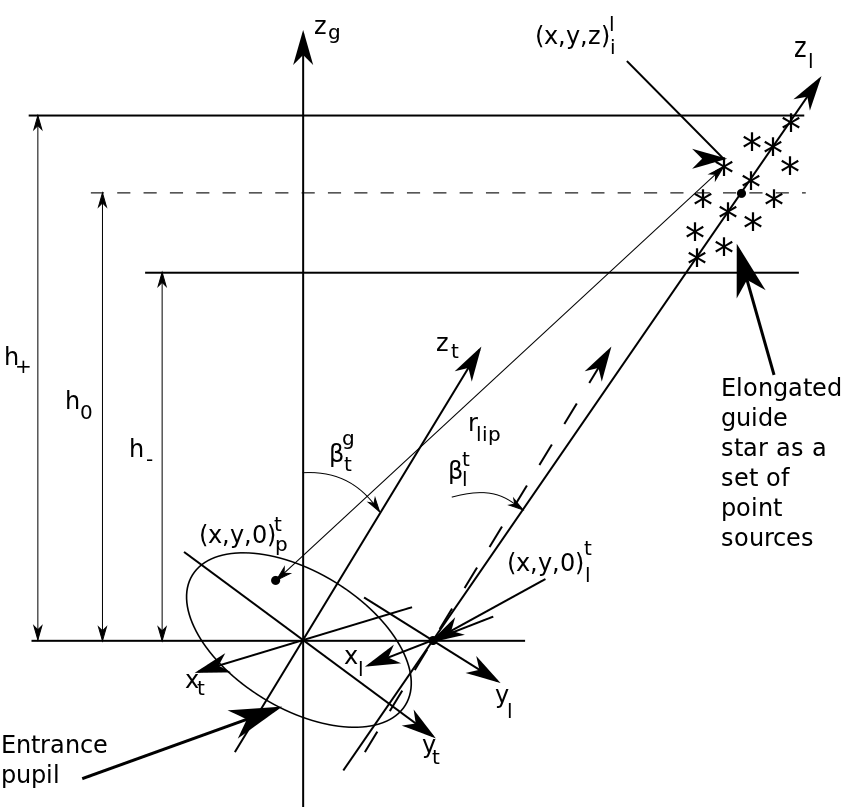
\includegraphics[width = 0.7\textwidth]{LGS.png}
\end{center}
\caption{Geometry of laser guide star propagation to the telescope entrance
pupil.}
\label{fig:lgs-geom}
\end{figure}

Three coordinate systems are involved:
\begin{enumerate}
	\item Global or $g$-system is the Cartesian coordinate system with respect
	to which all other coordinate systems are defined. The orientation pair
	$(\bm{o},\mathcal{R})_{g}^{0}$ for this system is just ($\bm{0},\mathcal{I}$).
	\item Telescope or $t$-system is the local Cartesian coordinate system
	rotating with respect to the $g$-system such that the $t$-system $z$-axis is
	always along the telescope optical axis. The orientation pair
	$(\bm{o},\mathcal{R})_{t}^{g}$ for this system describes the telescope
	pointing. If we assume that at zenith pointing the $t$-system coincides with
	the $g$-system, then \\
	\begin{equation} \label{eq:t-origin}
		\bm{o}^{g}_{t} = \bm{o}^{0}_{g} = \bm{0},
	\end{equation}
	\begin{equation} \label{eq:t-rotation}
		\mathcal{R}^{g}_{t} = \texttt{Eu}(\alpha^{g}_{t},\beta^{g}_{t},0),
	\end{equation}
	where Euler angles $\alpha^{g}_{t},\beta^{g}_{t}$ have meaning of the
	telescope azimuth and zenith angles measured with respect to the g-system
	(note the $g$ superscript). The standard Euler rotation is
	\begin{equation} \label{Euler}
		\texttt{Eu}(\alpha,\beta,\gamma) = \mathcal{A}_{z}(\alpha)
		                                   \mathcal{A}_{y}(\beta)
		                                   \mathcal{A}_{z}(\gamma),
	\end{equation}
	$$ \mathcal{A}_{z}(\alpha) = \left[
     \begin{array}{crc}
	     \cos{\alpha} & -\sin{\alpha} & 0 \\
	     \sin{\alpha} & \cos{\alpha} & 0 \\
	     0 & 0 & 1 \\
		 \end{array} \right],
	$$
	$$ \mathcal{A}_{y}(\beta) = \left[
     \begin{array}{rcc}
	     \cos{\beta} & 0 & \sin{\beta} \\
	     0 & 1 & 0 \\
	     -\sin{\beta} & 0 & \cos{\beta} \\
		 \end{array} \right].
	$$
	Coordinates of point $p$ in the entrance pupil given in $t$-system are
	$[x,y,0]_{p}^{t} = \bm{r}_{p}^{t}$.
	\item Laser launch telescope or $l$-system is a local Cartesian coordinate
	system chosen such that its $z$-axis is always along the optical axis of the
	LLT. This system is naturally defined with respect to the $t$-system because
	the LLT is mounted on the moving main telescope mount:
	\begin{equation} \label{eq:l-system}
		(\bm{o},\mathcal{R})_{l}^{t} = ([x,y,0]_{l}^{t},
                                 \texttt{Eu}(\alpha_{l}^{t},\beta_{l}^{t},0),
	\end{equation}
	where $[x,y,0]_{l}^{t} = \bm{r}_{l}^{t}$ are the $l^{th}$ LLT location in
	$t$-system (pupil
	coordinates), $\alpha_{l}^{t},\beta_{l}^{t}$ are the azimuth and zenith
	angles of the LLT orientation with respect to the main telescope optical
	axis. Note that, for simplicity, we count one LGS per one LLT. In reality
	one LLT of GMT will generate a pair of LGSs. To account for this we simply
	assume that there are two differently oriented virtual LLTs at the location
	of one real LLT.

	The LGS is modeled as a combination of the point sources (PSR) distributed
	within the \texttt{Na} layer. Coordinates
	$\bm{r}_{li}^{l}, \,\, l =
	1,...,\#LLT, \,\, i=1,...,\#PSR$ of the sources are given in the $l$-system.
\end{enumerate}

Given orientation pair $(\bm{o},\mathcal{R})_{b}^{a}$ defining $b$-system
coordinates with respect to $a$-system coordinates, the transformation of
coordinates written in $b$-system into the same coordinates written in
$a$-system is the \emph{direct affine transform}: \index{affine transform}
\begin{equation} \label{eq:direct-affine}
	\bm{r}^{a} = \mathcal{R}_{b}^{a} \bm{r}^{b} + \bm{o}_{b}^{a}.
\end{equation}
Correspondingly, the \emph{inverse affine transform} gives the coordinates
written in $b$-system from the ones written in $a$-system:
\begin{equation} \label{eq:inverse-affine}
	\bm{r}^{b} = (\mathcal{R}_{b}^{a})^{T} (\bm{r}^{a} - \bm{o}_{b}^{a}).
\end{equation}


\subsection{Finding LGS spot elongation and orientation on the detector}
\label{sec:elongation-orientation}

An important geometrical calculation needed for the theoretical evaluation of
the detector noise covariance matrix is to find the parameters of the
elongated LGS image in the detector focal plane.

Let a LGS is produced as a light-emitting column of length $L$ inside the
\texttt{Na} layer. We need to find the length of its image in the
Shack-Hartmann WFS focal plane behind a lenslet with location $\bm{r}^{t}_{l}$
(in the $t$-system)
projected on the telescope entrance pupil and the image orientation with
respect to the detector pixel grid. Let the beginning and end of the LGS light
column have $t$-system coordinates $\bm{r}^{t}_{1}$ and $\bm{r}^{T}_{2}$,
respectively. Consider vectors $\bm{r}^{t}_{1t} =
\bm{r}^{t}_{1}-\bm{r}^{t}_{l}$ and $\bm{r}^{t}_{2t} =
\bm{r}^{t}_{2}-\bm{r}^{t}_{l}$. Then, up to a scaling factor and a possible
mirror flip, the LGS
image on the detector is determined by a $(\varepsilon,\theta)$-pair, where
$\varepsilon$ is the angular size of the LGS column as seen from the lenslet
center $\bm{r}_{l}^{t}$, that is, the angle between vectors $\bm{r}^{t}_{1l}$
and $\bm{r}^{t}_{2l}$, and $\theta$ is the angle
between the $t$-system x-axis and the line of intersection of the $t$-system
xy-plane and the plane made by vectors $\bm{r}^{t}_{1l}$ and $\bm{r}^{t}_{2l}$.
Vectors $\bm{r}_{1,2}$ are most conveniently definable in the $l$-system,
where
\begin{equation} \label{eq:lgs-ends-l}
	\bm{r}^{l}_{1,2} = [0 \, 0 \, z^{l}_{1,2}]^{T}.
\end{equation}
The transformation to $t$-system is
\begin{equation} \label{eq:lgs-ends-t}
	\bm{r}^{t}_{1,2} = \mathcal{R}^{t}_{l} \bm{r}^{l}_{1,2} + \bm{o}^{t}_{l}.
\end{equation}
Using scalar and vector products we get
\begin{eqnarray} \label{eq:epsilon-theta}
	\hat{\bm{r}}^{t}_{1,2} = \frac{\bm{r}^{t}_{1,2}}{|\bm{r}^{t}_{1,2}|}, \\
	\cos \varepsilon = \hat{\bm{r}}^{t}_{1} \cdot \hat{\bm{r}}^{t}_{2}, \\
	\bm{p}^{t}_{12} = \hat{\bm{r}}^{t}_{1} \times \hat{\bm{r}}^{t}_{2}, \\
	\sin \varepsilon = |\bm{p}^{t}_{12}|, \\
	\hat{\bm{p}}^{t}_{12} = \frac{\bm{p}^{t}_{12}}{\sin \varepsilon}, \\
	\hat{\bm{x}}^{t} = [1 \, 0 \, 0]^{T}, \\
	\cos \theta = \hat{\bm{x}}^{t} \cdot \hat{\bm{p}}^{t}_{12}, \\
  \sin \theta = | \hat{\bm{x}}^{t} \times \hat{\bm{p}}^{t}_{12} |.
\end{eqnarray}
Note that, since $\varepsilon$ is very small, in order to preserve accuracy,
all calculations need to be done in double precision.

\subsection{Free-space propagation from LGS to telescope entrance pupil}
\label{sec:free-space-propagation}

The electric field $E$ from the LGS on the telescope entrance pupil is the
superposition of spherical waves emitted from each point source (PS) that
makes the elongated laser guide star spot in the \texttt{Na} layer:
\begin{equation} \label{eq:spherical-superposition}
	E_{lp} = \sum_{i=1}^{\#PSR} w_{li} \frac{\exp(i k r_{lip})}{r_{lip}},
\end{equation}
where $w_{li}$ is the weight describing relative intensity of the $i^{th}$ PS
of the $l^{th}$ LGS, $r_{lip}$ is the distance from the $i^{th}$ PS
of the $l^{th}$ LGS to $p^{th}$ point in the telescope entrance pupil. This
distance is easily found through the affine transform:
\begin{equation} \label{eq:source-to-pupil}
	\bm{r}_{li}^{t} = \mathcal{R}_{l}^{t} \bm{r}_{li}^{l} + \bm{o}_{l}^{t},
\end{equation}
$$ r_{lip} = |\bm{r}_{li}^{t} - \bm{r}_{p}^{t}|. $$

\subsection{Geometrical optics propagation through atmosphere}
\label{sec:geom-propagation}

The turbulent atmosphere on the way between an LGS and a telescope is modeled
as a set of infinitely thin random \emph{phase screens} (PS)
\index{phase screen}. Because of small phase perturbations caused by each
layer and because the typical scale of turbulence is much larger than a
wavelength the geometrical optics model for propagation through the layers is
assumed. The model is based on the following postulates:
\begin{itemize}
	\item The propagation of the electromagnetic waves is treated as propagation
	of \emph{rays} that are normals to the constant phase surfaces of the waves,
	the \emph{wavefronts}. \index{ray} \index{wavefront}
	\item Rays are always straight: the phase screens are weak enough for not
	to change direction of rays, they only add a path difference
	$\delta r_{lip,j}$:
	\begin{equation} \label{eq:path-diff}
		\delta r_{lip,j} = \phi_{lip,j}/k, \,\, j = 1,...,\#PS,
	\end{equation}
	$$ r_{lip}^{turb} = r_{lip}^{free} + \sum_{j=1}^{\#PS} \delta r_{lip,j}. $$
	where $\phi_{lip,j}$ is the phase on the $j^{th}$ turbulent layer
	intersected by a ray emitting from $i^{th}$ point source of $l^{th}$ LGS
	towards $p^{th}$ point in the entrance pupil. So, the electric field
	on the entrance pupil will be
	\begin{equation} \label{eq:spherical-superposition-turb}
		E^{turb}_{lp} =
		\sum_{i=1}^{\#PSR} w_{li}
		\frac{\exp(i k r_{lip}^{turb})}{r_{lip}^{free}}.
	\end{equation}
\end{itemize}

Thus, it is necessary to find the intersection of a ray with a turbulent layer.

\subsubsection{Turbulence layers are perpendicular to the telescope optical
axis.}

Assume that the turbulence layers are chosen such that they are perpendicular
to the telescope optical axis regardless of the pointing.
In this case the turbulence strength depends on the azimuth angle
$\beta_{t}^{g}$, namely,
\begin{equation} \label{eq:turb-vs-beta}
	C_{n}^{2} (\beta_{t}^{g}) = \frac{C_{n}^{2}(0)} {\cos \beta_{t}^{g}}.
\end{equation}

Simple geometrical analysis gives for the
relationship between the pupil and turbulence layer coordinates:
\begin{equation} \label{eq:pupil-to-layer}
  \bm{r}^{t}_{lip,j} =
  \frac{h_{j}}{z^{t}_{li}} \bm{r}_{p}^{t} +
  (1-\frac{h_{j}}{z^{t}_{li}})
  \left[
  \begin{array}{c}
	  x^{t}_{li} \\
	  y^{t}_{li} \\
	  0
	\end{array}
  \right], \,\,
  \bm{r}^{t}_{li} =
  \left[
  \begin{array}{c}
	  x^{t}_{li} \\
	  y^{t}_{li} \\
	  z^{t}_{li}
	\end{array}
  \right],
\end{equation}
where $h_{j}$ is distance between the telescope and $j^{th}$ phase screen
along the telescope optical axis,
$\bm{r}^{t}_{lip,j}$ are xyz-coordinates in $t$-system of an
intersection point on phase screen $j$ for a ray emitting from $i^{th}$ point
source of $l^{th}$ LGS with $t$-coordinates $\bm{r}^{t}_{li}$ and
passing through $p^{th}$ point in telescope entrance pupil with $t$-coordinates
$\bm{r}^{t}_{p}$. For the source at infinity (a natural guide star or a
scientific target) Eq. (\ref{eq:pupil-to-layer}) simplifies to
\begin{equation} \label{eq:pupil-to-layer-inf}
	\bm{r}^{t}_{lip,j} =
	\left[
	\begin{array}{c}
		\cos \alpha^{t}_{li} \\
		\sin \alpha^{t}_{li} \\
		0 \\
	\end{array}
	\right] h_{j} \tan \beta^{t}_{li} + \bm{r}^{t}_{p},
\end{equation}
where $(\alpha,\beta)^{t}_{li}$ are the angular coordinates (first and second
Euler angles) of the light source. Note that in both cases the position of the
ray intersection with a layer can be written as $ (a \bm{r}_{p}^{t} +
\bm{b}^{t}_{li}) $.

\subsubsection{Turbulence layers are parallel to the ground.}

Assume that the layers are parallel to the ground, i.e. perpendicular to the
$g$-system's $z$-axis, and have altitudes $h_{j}, \,\, j = 1,...,\#PS$. In
this case the turbulence $C_{n}^{2}$ profile is not altered with the zenith
angle. Direct ray tracing technique is used to find intersection with a
turbulence layer.

Coordinates of a ray can be described through the parametric equation:
\begin{equation} \label{eq:ray-equation}
	\bm{r}(t) = \bm{i} t + \bm{r}_{0},
\end{equation}
where $\bm{r}_{0}$ is the ray origin (position of the light-emitting source),
$\bm{i}$, $|\bm{i}| = 1$ is the ray
direction vector, $t$ is the ray path length. In the case of propagation path
shown of Fig. \ref{fig:lgs-geom}
$$ \bm{r}^{l}_{0} = \bm{r}^{l}_{li}, $$
where $\bm{r}_{0}$ is given in $l$-system,
$$ \bm{i}^{t} = \frac{\bm{r}^{t}_{p} - \bm{r}^{t}_{li}}
                 {|\bm{r}^{t}_{p} - \bm{r}^{t}_{li}|}, $$
where $\bm{i}$ is given in $t$-system. Since the turbulent layers are most
conveniently defined in the $g$-system, the ray coordinates need to be
transformed into $g$-system:
\begin{equation} \label{eq:ray-transform}
	\bm{r}^{t}_{0} = \mathcal{R}_{l}^{t} \bm{r}^{l}_{0} + \bm{o}_{l}^{t},
\end{equation}
$$ \bm{i}^{t} = \frac{\bm{r}^{t}_{p} - \bm{r}^{t}_{0}}
                 {|\bm{r}^{t}_{p} - \bm{r}^{t}_{0}|}, $$
$$ \bm{r}^{g}_{0} = \mathcal{R}_{t}^{g} \bm{r}^{t}_{0} + \bm{o}_{t}^{g}, $$
$$ \bm{i}^{g} = \mathcal{R}_{t}^{g} \bm{i}^{t}. $$
The coordinates of ray intersection with turbulent layer are found by equating
$z$-coordinate of a ray to the layer altitude:
\begin{equation} \label{eq:layer-intersection}
	t = \frac{h_{j}-r^{g}_{0z}}{i^{g}_{z}},
\end{equation}
$$ \bm{r}^{g}_{lip,j} = \bm{i}^{g} t + \bm{r}_{0}^{g}, $$
where $x$- and $y$-coordinates of the $\bm{r}^{g}_{lip,j}$-vector are used to
find the phase $\phi^{turb}(\bm{r}^{g}_{lip,j}) = k \delta r^{turb}_{lip,j}
(\bm{r}^{g}_{lip,j})$ on the phase
screen corresponding to the ray intersection and substitute it to Eq.
(\ref{eq:spherical-superposition-turb}).


\subsection{Point source distribution in the LGS}
\label{sec:point-distribution}
TBC

The positions $\bm{r}^{l}_{li}$ and weights $w_{li}$ of point sources making
each LGS are found from superposition of the intensity distribution of the laser
radiation forward-propagated through atmosphere to the \texttt{Na} layer and
the vertical distribution of the \texttt{Na} density. A possible operation
flow for defining the LGS distribution is the following:
\begin{enumerate}
	\item Define a 3D mesh covering a part of the \texttt{Na} layer penetrated
	by the laser radiation. Each cell of this mesh is an elementary volume for
	which amount of laser flux is assigned.
	\item Center of each 3D mesh cell is the candidate location of the LGS point
	source. If flux through the cell exceeds a threshold, a point source is
	assigned for this cell.
	\item For each mesh cell for which a point source is assigned multiply the
	cell flux by \texttt{Na} density at the cell center taken from the
	\texttt{Na} vertical profile. Find relative distribution of the return flux,
	which is the source weights $\{ w_{li} \}_{i=1}^{\#PSR}$:
	\begin{equation} \label{eq:source-weights}
		w_{li} = \frac{ \Phi_{li} C^{\texttt{Na}}_{li} }
		               { \sum_{i=1}^{\#PSR} \Phi_{li} C^{\texttt{Na}}_{li} },
		           \,\, i = 1, ... , \#PSR
	\end{equation}
	where $\{ \Phi_{li} \}_{i=1}^{\#PSR}$ are the cell fluxes,
	$\{ C^{\texttt{Na}}_{li} \}_{i=1}^{\#PSR}$ are the \texttt{Na} abundances at
	the cell locations.
\end{enumerate}

\subsection{Return flux in the entrance pupil}
\label{sec:return-flux}

The photon flux returning from each LGS point source is considered uniformly
distributed over the spherical surface of the wavefront. Since the solid angle
$\Omega$ at which the telescope is seen from the source is typically very
small, the variation of $r^{free}_{lip}$ in the denominator of Eq.
(\ref{eq:spherical-superposition-turb}) over the pupil can be neglected. Thus,
the fraction of energy emitting from a point source that passes through the
telescope entrance pupil is
\begin{equation} \label{eq:energy-fraction}
	\frac{\Omega}{4 \pi} = \frac{1}{4 \pi}
	\frac{ A_{p} }
	     { |\bm{r}^{t}_{li}|^{2} \cos^{2} \beta^{t}_{li} },
\end{equation}
where $A_{p}$ is the pupil area, $|\bm{r}^{t}_{li}|$ is the distance from
pupil center to the point source, $\beta^{t}_{li}$ is the angle between the
telescope optical axis and the direction to the point source as seen from the
pupil center,
\begin{equation} \label{eq:angle-to-source}
	\cos \beta^{t}_{li} = \left( \frac{\bm{r}^{t}_{li}}
	                                  {|\bm{r}^{t}_{li}|} \right)_{z}.
\end{equation}
The photon flux into the entrance pupil from a point source is
\begin{equation} \label{eq:return-flux}
	\Phi_{li} = \tau T_{AOS} \frac{T_{ATM}}{\cos{\beta^{g}_{li}}}
	            s^{\texttt{Na}} C^{\texttt{Na}}
	            P_{l} w_{li}
	            \frac{\Omega}{4 \pi}, \,\, [\texttt{photons}],
\end{equation}
where \\
\begin{tabular}{lcll}
	&&& \\
  Exposure time & : & $\tau$ & = 2 ms, \\
  Atmosphere transmittance & : & $T_{ATM}$ & = 0.89, \\
  AO system transmittance & : & $T_{AOS}$ & = 0.448, \\
  Sodium coupling efficiency & : & $s^{\texttt{Na}}$ &
  = 130 (photons m$^{2}$ )/(s W atom), \\
  Sodium abundance & : & $C^{\texttt{Na}}$ & = $2.1\times10^{13}$ atoms/m$^2$,\\
	Laser power per LGS & : & $P_{l}$ & = 20 W, \\
	&&& \\
\end{tabular} \\
$\beta^{g}_{li}$ is the angle between zenith direction and the point source
direction as viewed from the entrance pupil center.

The fluxes from all point sources are later summed on the detector.